%%%%%%%%%%%%%%%%%%%%%%%%%%%%%%%%%%%%%%%%%%%%%%%%%%%%%%%%%%%%%%%%%%%%%%%%%%%%%%%%%%%%%%%
%%%%%%%%%%%%%%%%%%%%%%%%%%%%%%%%%%%%%%%%%%%%%%%%%%%%%%%%%%%%%%%%%%%%%%%%%%%%%%%%%%%%%%%
%%%%%%%%%%%%%%%%%%%%%%%%%%%%%%%%%%%%%%%%%%%%%%%%%%%%%%%%%%%%%%%%%%%%%%%%%%%%%%%%%%%%%%%
\section{Regressão polinomial múltipla com $\VECTOR{h}(x,y):~\mathbb{R}^2 \rightarrow \mathbb{R}^2$}
\label{sec:theo:maphxr2r2}

\index{Problema inverso: Aplicado!Linear}
\index{Regressão não linear!Múltipla!Polinômio $\VECTOR{h}(x,y):~\mathbb{R}^2 \rightarrow \mathbb{R}^2$}
\index{Regressão!Polinômio $\VECTOR{h}(x,y):~\mathbb{R}^2 \rightarrow \mathbb{R}^2$}

\begin{theorem}[Regressão usando um polinômio 
$\VECTOR{f}(x,y):$ $\mathbb{R}^2 \rightarrow \mathbb{R}^2$, de grau $M$:]
\label{theo:maphxr2r2}
~\\
\begin{minipage}{0.45\textwidth}
\centering
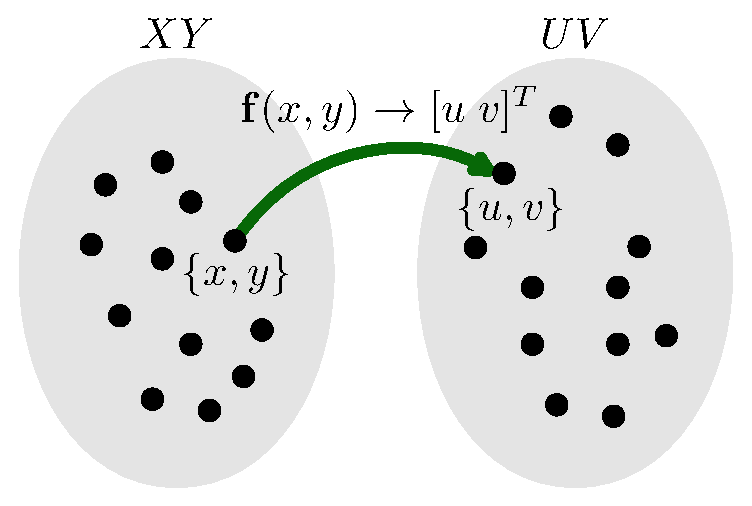
\includegraphics[width=0.85\linewidth]{chapters/mapeamento/mapeamento.eps} 
\end{minipage}
\begin{minipage}{0.55\textwidth}
Dados
os escalares 
$x \in \mathbb{R}$, 
$y \in \mathbb{R}$, 
$u \in \mathbb{R}$ e 
$v \in \mathbb{R}$,
os vetores $\VECTOR{c} \in \mathbb{R}^{\frac{(M+1)(M+2)}{2}}$ e
$\VECTOR{d} \in \mathbb{R}^{\frac{(M+1)(M+2)}{2}}$,
com elementos $c_k$ e $d_k$,
uma função polinomial $\VECTOR{h}:\mathbb{R}^2 \rightarrow \mathbb{R}^2$, de grau $M$, e 
definida a Eq. (\ref{eq:maphxr2r2:1}),
\begin{equation}\label{eq:maphxr2r2:1}
\begin{bmatrix}
u\\
v
\end{bmatrix} =
\VECTOR{h}(x,y) \equiv 
\begin{bmatrix}
h_{\VECTOR{c}}(x,y)\\
h_{\VECTOR{d}}(x,y)
\end{bmatrix}
\end{equation}
\end{minipage}
\noindent
\begin{equation}\label{eq:maphxr2r2:1a}
h_{\VECTOR{c}}(x,y) = \sum \limits_{m=0}^{M} \sum \limits_{l=0}^{m}c_{\left\{ \frac{m(m+1)}{2}+l+1\right\}}~x^{m-l}y^{l}, 
~~~
h_{\VECTOR{d}}(x,y) = \sum \limits_{m=0}^{M} \sum \limits_{l=0}^{m}d_{\left\{ \frac{m(m+1)}{2}+l+1\right\}}~x^{m-l}y^{l}; 
\end{equation}
%\begin{equation}\label{eq:maphxr2r2:1b}
%\end{equation}
podemos afirmar que os vetores coluna $\VECTOR{c}=\VECTOR{\hat{c}}$ e
$\VECTOR{d}=\VECTOR{\hat{d}}$,
que minimizam os erros $e_{\VECTOR{c}}(\VECTOR{c})$ e $e_{\VECTOR{d}}(\VECTOR{d})$,
respetivamente,
\begin{equation}\label{eq:maphxr2r2:2}
%e(\VECTOR{c}) = ||h(\VECTOR{x})-\VECTOR{y}||_{\MATRIX{W}}^2 \equiv \sum_{n=1}^{N} w_n||h(x_n)-y_n||^2,
e_{\VECTOR{c}}(\VECTOR{c}) =  \sum_{n=1}^{N} w_n||h_{\VECTOR{c}}(x_n,y_n)-u_n||^2,\qquad 
e_{\VECTOR{d}}(\VECTOR{d}) =  \sum_{n=1}^{N} w_n||h_{\VECTOR{d}}(x_n,y_n)-v_n||^2,
\end{equation}
proveniente de avaliar $N$ amostras $\{x_n,y_n\}$ e $\{u_n,v_n\}$ 
que não cumprem necessariamente a Eq. (\ref{eq:maphxr2r2:1}), 
representadas pelos vetores 
$\VECTOR{x}=[x_1~ ...~ x_n~ ...~ x_N]^{\transpose}$,
$\VECTOR{y}=[y_1~ ...~ y_n~ ...~ y_N]^{\transpose}$, 
$\VECTOR{u}=[u_1~ ...~ u_n~ ...~ u_N]^{\transpose}$, e
$\VECTOR{v}=[v_1~ ...~ v_n~ ...~ v_N]^{\transpose}$,
ponderadas com os pesos $w_n \in \mathbb{R}_+$, 
representados pela matriz diagonal $\MATRIX{W}=\funcdiag([w_1~ w_2~ ...~ w_n~ ...~ w_N]^{\transpose})$;
podem ser achados\footnote{A demonstração pode ser vista na Prova \ref{proof:theo:maphxr2r2}.} usando:
\begin{equation}\label{eq:maphxr2r2:3}
\VECTOR{\hat{c}}=
\left[ \MATRIX{A}^{\transpose} \MATRIX{W} \MATRIX{A} \right]^{-1}\MATRIX{A}^{\transpose} \MATRIX{W} \VECTOR{u},
\qquad \qquad \qquad \qquad
\VECTOR{\hat{d}}=
\left[ \MATRIX{A}^{\transpose} \MATRIX{W} \MATRIX{A} \right]^{-1}\MATRIX{A}^{\transpose} \MATRIX{W} \VECTOR{v}.
\end{equation}
onde a matriz $\MATRIX{A}$ é definida como,
\begin{equation}\label{eq:maphxr2r2:4}
\MATRIX{A}\equiv\MATRIX{A}(\VECTOR{x},\VECTOR{y})=\begin{bmatrix}
\VECTOR{a}(x_1,y_1)\\
\VECTOR{a}(x_2,y_2)\\
\vdots\\
\VECTOR{a}(x_N,y_N)\\
\end{bmatrix}, \qquad
\begin{matrix}
\VECTOR{a}(x,y)= &
\begin{bmatrix}
\VECTOR{s}_{0}(x,y) & \VECTOR{s}_{1}(x,y) &  \dots  & \VECTOR{s}_{M}(x,y)
\end{bmatrix},\\
~&~\\
\VECTOR{s}_{m}(x,y)=&
\begin{bmatrix}
x^m  & x^{m-1} y  & x^{m-2} y^2    & \dots  & x y^{m-1} &  y^m 
\end{bmatrix}.
\end{matrix}
\end{equation}


\end{theorem}

\begin{tcbattention}
\begin{itemize}
\item Uma forma de reescrever a Eq. (\ref{eq:maphxr2r2:1a}) usando a Eq. (\ref{eq:maphxr2r2:4}) é:
\begin{equation}\label{eq:maphxr2r2:5}
h_{\VECTOR{c}}(x,y) = \VECTOR{a}(x,y)\VECTOR{c}, 
\qquad
h_{\VECTOR{d}}(x,y) = \VECTOR{a}(x,y)\VECTOR{d}; 
\end{equation}

\item É importante lembrar que para que os vetores $\VECTOR{c}$ e $\VECTOR{d}$
que minimizam $e(\VECTOR{c})$ e $e(\VECTOR{d})$ tenham resposta única,
é necessário (porém não suficiente) que o número de amostras $N$ seja maior ao número de colunas de $A$;
quer dizer $N\geq \frac{(M+1)(M+2)}{2}$.

\item De forma exata, podemos afirmar que para que os $\VECTOR{c}$ e  $\VECTOR{d}$ tenham resposta única,
deve existir inversa para a matriz $\MATRIX{A}^{\transpose}\MATRIX{W}\MATRIX{A}$.

\end{itemize}
\end{tcbattention}


%%%%%%%%%%%%%%%%%%%%%%%%%%%%%%%%%%%%%%%%%%%%%%%%%%%%%%%%%%%%%%%%%%%%%%%%%%%%%%%%
\subsection{Exemplos de regressão com um polinômio
$\VECTOR{h}(x,y):~\mathbb{R}^2 \rightarrow \mathbb{R}^2$ de grau $M$}

\begin{example}[ Regressão do polinômio 
$\VECTOR{h}(x,y)$ de grau $M=3$, para $N=15$ amostras:]\label{ex:theo:mapeamentor2r2}
Dadas $N=15$ amostras que representam pontos no plano $XY$ e seus correspondentes 
no plano $UV$, como pode ser visto na Tabela \ref{table:ex:mapeamentor2r2},
obter a função polinomial $\VECTOR{h}(x,y)=[h_{\VECTOR{c}}(x,y)\quad h_{\VECTOR{d}}(x,y)]^{\transpose}$ de grau $M=3$,
que mapeia com o menor erro $e_{\VECTOR{c}}(\VECTOR{c})$ e $e_{\VECTOR{d}}(\VECTOR{d})$, 
ambos conjuntos de pontos.
\end{example}

\noindent
\begin{minipage}{0.4\textwidth}
\centering
\begin{minipage}{0.9\textwidth}
\begin{table}[H]%[h!]
\centering
\begin{tabular}{ |r |r || r |r|}
\hline
   $\VECTOR{x}$ & $\VECTOR{y}$ & $\VECTOR{u}$ & $\VECTOR{v}$ \\ \hline \hline
  -0.81 &-0.69 &-0.44 & 1.09 \\ 
   0.75 & 0.02 & 0.20 &-0.76 \\ 
   0.47 & 0.67 & 0.73 &-0.46 \\ 
   0.66 &-0.25 &-0.07 &-0.66 \\ 
  -0.76 & 0.73 &-0.91 &-0.63 \\ 
   0.10 &-0.72 &-0.50 & 0.20 \\ 
  -0.43 &-0.85 &-0.55 & 0.84 \\ 
   0.91 &-0.92 &-0.78 &-0.16 \\ 
   0.64 &-0.76 &-0.61 &-0.12 \\ 
  -0.79 &-0.28 &-0.35 & 0.46 \\ 
   1.00 &-0.27 & 0.08 &-0.75 \\ 
   0.84 &-0.11 & 0.13 &-0.75 \\ 
   0.79 & 0.95 & 1.79 & 0.79 \\ 
   0.65 &-0.90 &-0.82 & 0.06 \\ 
   0.76 &-0.95 &-0.88 & 0.03 \\ \hline
\end{tabular}
\caption{Valores $\{x_n,y_n\}$ do plano $XY$ e valores $\{u_n,v_n\}$ do plano $UV$.}
\label{table:ex:mapeamentor2r2}
\end{table}
\end{minipage}
\end{minipage}
\begin{minipage}{0.6\textwidth}
\begin{SolutionT}[Relativa ao Exemplo \ref{ex:theo:mapeamentor2r2}:]\label{sol:theo:mapeamentor2r2}
Se desejamos obter a função polinomial $\VECTOR{f}(x,y)$ de grau $M=3$,
que mapeia os conjuntos de pontos $\{x_n,y_n\}$ e $\{u_n,v_n\}$ da Tabela \ref{table:ex:mapeamentor2r2}; 
podemos usar a Eq. (\ref{eq:maphxr2r2:3}) 
para obter os vetores $\VECTOR{c}=\VECTOR{\hat{c}}$ e $\VECTOR{d}=\VECTOR{\hat{d}}$,
que minimizam $e_{\VECTOR{c}}(\VECTOR{c})$ e $e_{\VECTOR{d}}(\VECTOR{d})$.


Assim, usando a Eq. (\ref{eq:maphxr2r2:3}), obtemos o vetor $\VECTOR{\hat{c}}=$ 
\begin{center}
\begin{tabular}{ r r r r }
  \hline
  -0.060306 &   0.240624 &   0.260580 &  -0.117630 \\ \hline
   0.996594 &  -0.089543 &   0.304348 &  -0.128405 \\ \hline
   0.464804 &   0.481949 & ~ & ~ \\ \hline
\end{tabular}
\end{center}

e o vetor $\VECTOR{\hat{d}}=$ 
\begin{center}
\begin{tabular}{ r r r r }
\hline
  -0.70762 &  -0.37822 &  -0.96840 &   0.57036 \\ \hline
   0.90987 &   0.83260 &  -0.21166 &   0.49152  \\ \hline
   0.55825 &   0.39762 & ~ & ~ \\ \hline
\end{tabular}
\end{center}
Esses vetores provocam um erro 
de $e_{\VECTOR{c}}(\VECTOR{c})=5.6808e-05$ e $e_{\VECTOR{d}}(\VECTOR{d})=1.4242e-05$, respetivamente.
Podem ser vistos gráficos das superfícies $h_{\VECTOR{c}}(x,y)$ e $h_{\VECTOR{d}}(x,y)$ 
do Exemplo \ref{ex:theo:mapeamentor2r2} na Figura \ref{fig:theo:maphxr2r1:xnynunvn}.
\end{SolutionT}
\end{minipage}

\begin{figure}[!h]
\centering
    \begin{subfigure}[b]{0.45\textwidth}
        \centering
        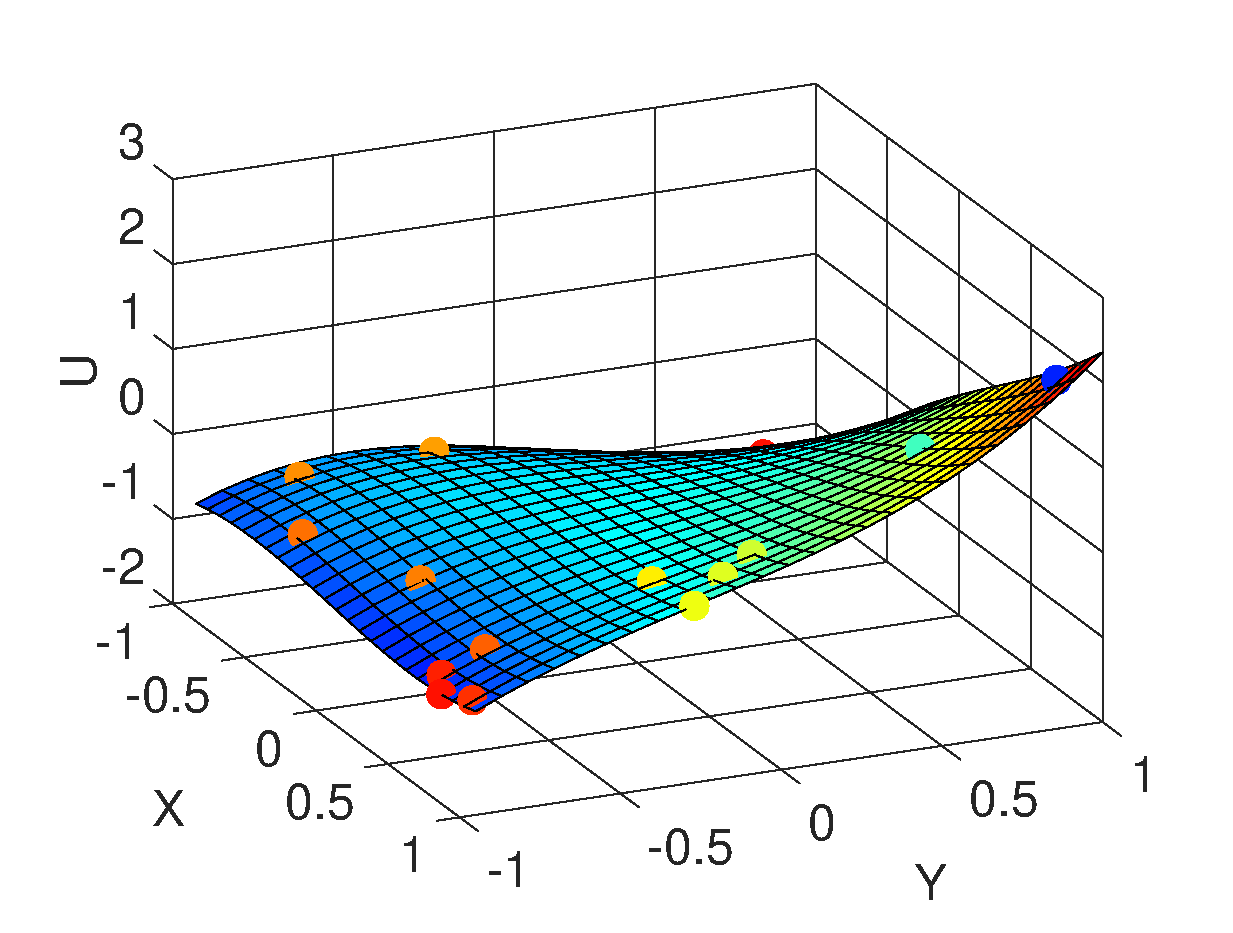
\includegraphics[width=\textwidth]{chapters/mapeamento/mfiles/mapeamentor2r2/minimizando_hxc.eps}
        \caption{Gráfico das amostras $\{x_n,y_n,u_n\}$ e da superfície $u=h_{\VECTOR{c}}(x,y)$.}
        \label{fig:theo:maphxr2r1:xnynun}
    \end{subfigure}
    ~
    \begin{subfigure}[b]{0.45\textwidth}
        \centering
        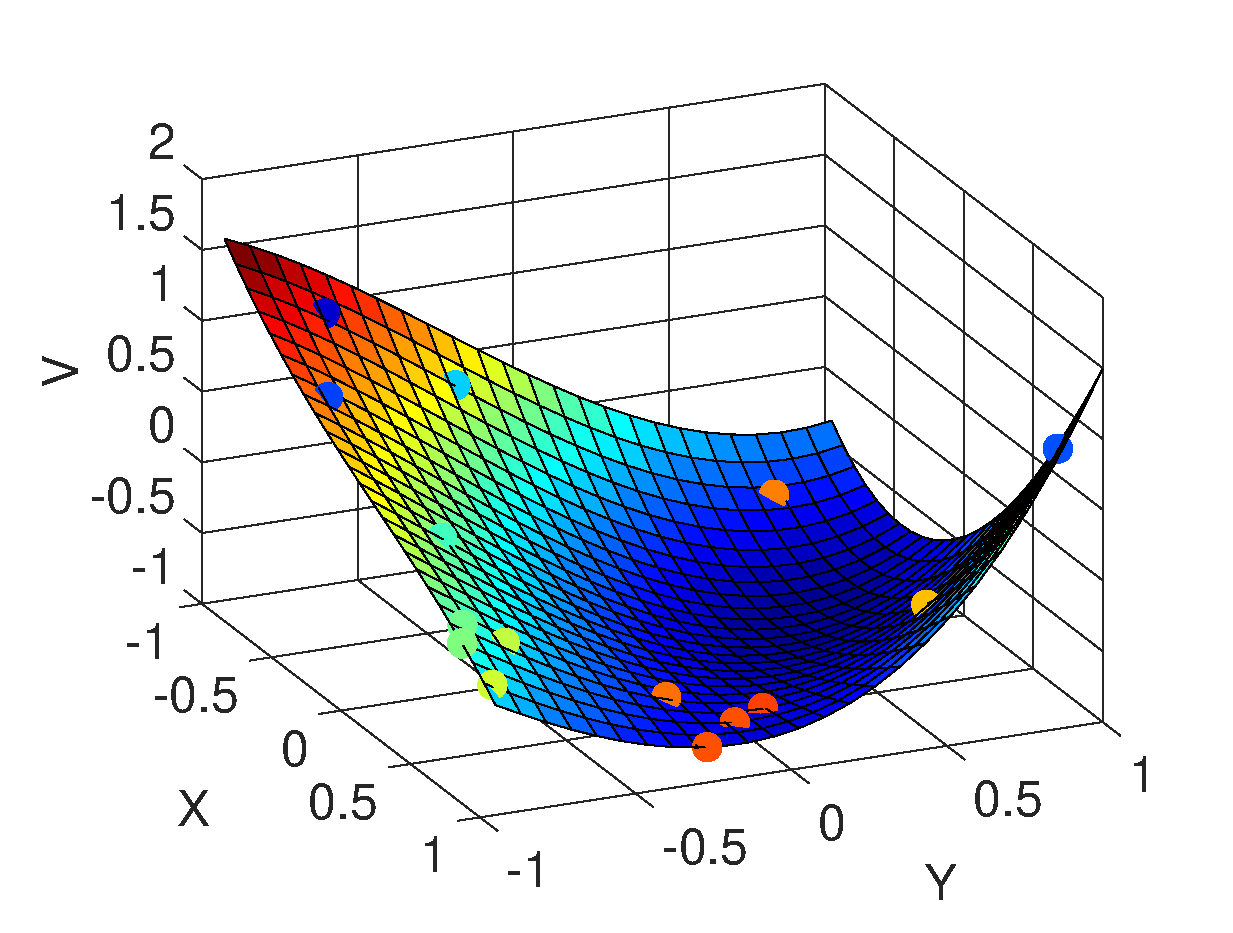
\includegraphics[width=\textwidth]{chapters/mapeamento/mfiles/mapeamentor2r2/minimizando_hxd.eps}
        \caption{Gráfico das amostras $\{x_n,y_n,v_n\}$ e da superfície $v=h_{\VECTOR{d}}(x,y)$.}
        \label{fig:theo:maphxr2r1:xnynvn}
    \end{subfigure}
\caption{Gráfico das superfícies do Exemplo \ref{ex:theo:mapeamentor2r2}.}
\label{fig:theo:maphxr2r1:xnynunvn}
\end{figure}
